\documentclass[a4paper]{article}
\usepackage[T1]{fontenc}
\usepackage[utf8]{inputenc}
%\usepackage[top=2cm, bottom=2cm, left=2cm, right=2cm]{geometry}
\usepackage{color}
\usepackage{minted}
\usepackage{url}
\usepackage{array}
\usepackage{pifont}
\usepackage{graphicx}
\setlength{\skip\footins}{2cm}


\newminted{java}{xleftmargin=1cm}
\usemintedstyle{trac}

\title{A component-based Distributed Information System}
\author{
Matthieu \textsc{Dubet} \\
Alexander \textsc{Kawrykow} \\ \\ \\
\emph{COMP512 Distributed Systems} \\
\emph{School of Computer Science, McGill University}
}

\begin{document}
\maketitle
\begin{figure}
  \centering
	
\includegraphics[scale=0.8]{mcgill_logo.png}
  \label{mcgill}
\end{figure}
\clearpage
\tableofcontents
\clearpage


\section{General Design}

\begin{figure}
  \centering
	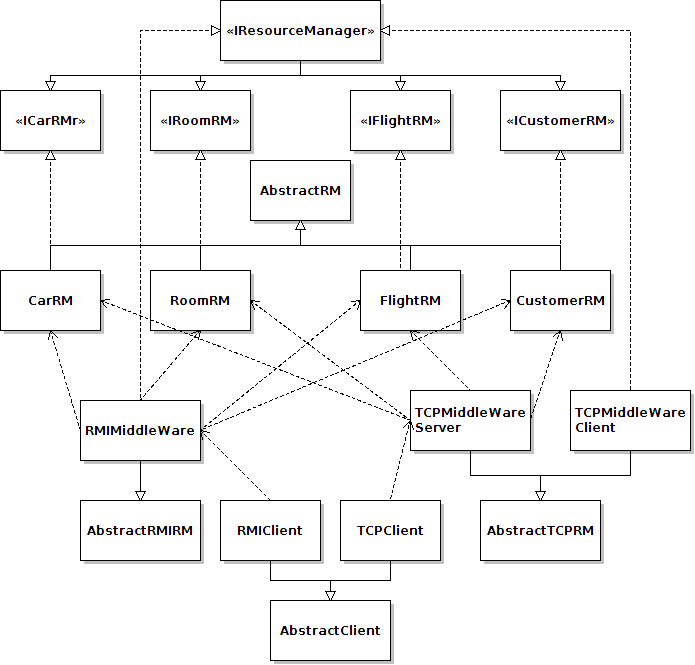
\includegraphics[scale=0.5,angle=90]{classhierarchy.png}
  \caption{UML Class Diagram}
  \label{uml}
\end{figure}

\subsection{Resource Manager}
We decided to separate the ResourceManager interface to split the concerns. 

Accordingly, we created one type of Interface for each kind of resource (room, car, flight, customer), and finally aggregated all these into one large interface (the \texttt{IResourceManager}). 


We then looked at the functionality common to anything Resource-Manager related: reading data, writing data, querying data, etc. In particular,
these are functions which have no semantic meaning specific to any of the resources. We extracted these into an \texttt{AbstractResourceManager}.
For each kind of resource, we implemented a concrete ResourceManager who was able to reuse the functionality in the AbstractResourceManager, but in the context of a particular resource (see Fig.\ref{uml} and \ref{carrm}).

 
\begin{figure}[h!]
  \centering
	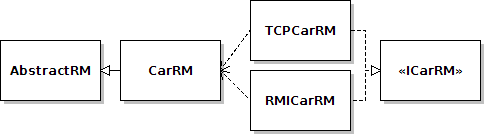
\includegraphics[scale=0.6]{carrm.png}
  \caption{ResourceManager hierarchy}
  \label{carrm}
\end{figure}

Both our RMI and TCP implementations of the ResourceManagers act as wrappers for their underlying ResourceManager. That is, a RMI car resource manager
takes care of binding to the registry and remote method calls, but the underlying logic happens by delegating to a concrete car resource manager. A
similar approach was taken for the TCP car resource manager. In this way, we were able to maximize code reuse. 


Another step taken to maximize code reuse was our treatment of the Client. Rather than re-writing the client for TCP, we created a TCP \emph{proxy} resource
manager which implements IResourceManager, but simply passes on the exact command to the remote middleware server. Here, the proxy is simply a local reference we can create when the client is launched.


The remote middleware server listens for the TCP/IP messages, looks at the first few letters, and then delegates the exact command. For example, we know a command containing the substring "car" must be sent, via TCP/IP, to the car resource manager server, so little processing of the commands ever needs to take place. 

The car resource manager can then just look at the first few letters of his received command,
and delegate to his reference to a local concret CarResourceManager depending on the type of query. For example, if the command starts with 'new', we know
we can call the newCar() method on the local reference and have him take care of the logic. 

\subsection{Customer Manager}

To handle customers, we decided to treat the MiddleWare as a kind of resource manager himself. 

The Middleware server has a local reference to a CustomerResourceManager object to handle all of the logic pertaining to customers, as well as reservations and the itinerary feature. In the case of RMI, the CustomerResourceManager can use his remote object references to easily handle reservations.

By contrast, for the TCP implementation, we had to reconstruct the objects the CustomerResourceManager would put in his hashtable. 
We did this by exchanging the objects over sockets in string form, as a list of attributes corresponding to the id, location, price, etc. For example, to reserve a car, the flow goes something like: send message to middleware, middleware constructs Car object by sending message to car resource manager to obtain the state of the specific car, middleware passes the car object to his local customer resource manager who places it in his hashtable to keep track of the reference. 

\subsection{Transaction Manager}
We noticed that we could support transaction support for \it both \rm TCP and RMI, \emph{for free}, if transaction management was implemented at the \texttt{CarRM} level. Accordingly, we defined a new interface \texttt{ITransactionManager} which 
exposes the set of methods prescribed in the assignment and had both \texttt{RMICarRM} and \texttt{TCPCarRM} implement this interface. Again, we maximized code reuse by delegating to the concrete \texttt{CarRM} for handling transactions
rather than redoing it for both TCP and RMI. Likewise, we noticed that the set of methods exposed by the \texttt{ITransactionManager} was exactly the same for all of the resource managers. That is, a \texttt{commit} always:

\begin{enumerate}
 \item Removes the transaction from the list of active transactions 
 \item Unlocks all resources held by that transaction
\end{enumerate}

Similarly, an \texttt{enlist} adds the transaction to the list of active transactions, while an \texttt{abort} always:

\begin{enumerate}
\item Does a rollback
\item Remove from active transaction list
\item Unlock resources.
\end{enumerate}

The data structures involved are the same regardless of resource manager type. Consequently, these methods were all implemented in \texttt{AbstractRM} and inherited by the concrete RMs. Adding transaction support then simply involved adding a few lines to each method of each RM:

\begin{enumerate}
 \item Check if the given \texttt{TxID} is in the list of active transactions, and throw an \texttt{InvalidTransactionException} if not
 \item For a write, load the appropriate UNDO op (see section \ref{rollbacks})
 \item Lock the resource, uniquely identified by the Key (for example, this key is the \texttt{location} parameter for the car RM).
\end{enumerate}

In this way, the middleware only needed to be modified slightly: upon receiving, for example, a query for a car's price, we call the remote car RM's method and only need to worry about catching the appropriate exceptions. For example, if a 
\texttt{DeadLockException} is thrown, we tell all RM's to abort. In this way, each resource manager worries only about locking their own kind of resource, rather than a centralized transaction manager worrying about all the resources.
Likewise, each resource manager has its own \texttt{LockManager} instance for locking, rather than a centralized lock manager. A glimpse of the updated design is provided in Figure \ref{txncarrm}.

To implement transaction timeout (a transaction which takes too much time before committing or aborting), we maintain a timer for each transaction, and each time an operation which is part of this transaction is received in the middleware, we restart the timer. When there is a timeout, we abort the transaction (thus maintaining data coherency thanks to rollbacks).

\begin{figure}[h!]
  \centering
	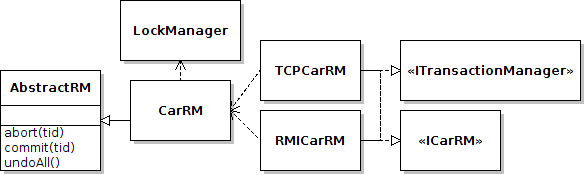
\includegraphics[scale=0.6]{txncarrm.png}
  \caption{ResourceManager hierarchy with transaction management}
  \label{txncarrm}
\end{figure}

\subsection{Replication and Fault-tolerance}

\subsubsection{Resource Manager}

There is two types of operations on a resource manager:
\begin{itemize}
\item
for a \texttt{READ} operation, the middleware forwards it to one of the concerned RMs, currently with a round-robin choice. If the operation doesn't succeed because of a RemoteException, then we assume that this RM is not available anymore. If there is still some RMs available, we recursively call the operation on the middleware, if no RM is available, we stop the system.

\begin{javacode}
    try {
      keepAlive(id);
      int rooms = roomRM.queryRooms(id, location);
      scheduleNextRoomRM();
      return rooms;
    } catch (InvalidTransactionException e) {
      Trace.error("[ERROR] "+e.getMessage());
    } catch (DeadlockException e) {
      System.out.println(this+"::DEADLOCK. Aborting txid "+id);
      abort(id);
    } catch (RemoteException e){
      // verify that there is still RMs available
      handleRoomRMCrash(roomRM);
      scheduleNextRoomRM();
      // retry the read
      if (roomRMs.size() > 0)
        return queryRooms(id, location);
    }    
\end{javacode}

\item
for a \texttt{WRITE} request, we have to forward the request to every concerned RMs currently active. We update them sequentially, and if the method call on a RM doesn't succeed, we take care of maintaining the data coherency by undoing the operation on the already updated RMs. Again, the handleRMCrash() method verify that there is still some available RMs, or stop the system.
\begin{javacode}
    keepAlive(id);
    for (int i = roomRMs.size() - 1; i >= 0; i--){
      try {
        success &= roomRMs.get(i).addRooms(id, location, numRooms, price);
        if (!success){
          for (int j = roomRMs.size() - 1; j > i; j--){
            roomRMs.get(j).undoLast(id);
          }
          break;
        }
      } catch (RemoteException e){
        handleRoomRMCrash(roomRMs.get(i));
      } catch (DeadlockException e) {
        System.out.println(this+":: DEADLOCK when adding room. txid: "+id);
        abort(id);
        success = false;
      } catch (InvalidTransactionException e) {
        Trace.error("[ERROR] "+e.getMessage());
        success = false;
      }
    }
\end{javacode}
\end{itemize}

\subsubsection{Middleware}
For the middleware fault-tolerance, we created a new class \emph{RMIMiddlewareGroupManager} (implements interface IMiddleware) which is the object called by the client. 
For every kind of request (\texttt{READ} or \texttt{WRITE}), the RMIMiddlewareGroupManager forwards the request to one actual middleware only! If the method call doesn't succeed, it tries on another middleware (and removes this middleware from the available middleware list).
\begin{javacode}
    try {
      success = middleware.addCars(id, location, numCars, price);
    } catch (RemoteException e){
      handleMiddlewareCrash(middleware);
      scheduleNextMiddleware();
      if (middlewares.size() > 0)
        return addCars(id, location, numCars, price);
    }	
    scheduleNextMiddleware();
\end{javacode}

\subsubsection{Recovery}

When a remote method call on a middleware or on a RM doesn't succeed (thus we assume that the server is not available anymore), we move this server from the active list to the recovery list.
Periodically, we ping every servers in the recovery list to put them back into the active list if the ping succeed, thus achieve some sort of server recovery.
Unfortunately, a bug
\footnote{http://bugs.sun.com/bugdatabase/view\_bug.do?bug\_id=4457683} in the implementation of \emph{unexport} method make the recovery not functional currently (as the port used for exporting the object isn't properly freed).
\subsection{Rollbacks}
\label{rollbacks}

A rollback consists of sequential execution of inverse operations. For example, the inverse of an \texttt{ADD} is a \texttt{DELETE} (and vice-versa), and the inverse of a \texttt{WRITE} is a \texttt{WRITE} containing the old values. 
We defined a generic \texttt{Operation} class which encapsulates this concept. Each instance of \texttt{Operation} contains a type (one of \texttt{ADD}, \texttt{DELETE}, \texttt{WRITE}, \texttt{UNRESERVE}) as well as a key-value pair
which describes the operation. For example, an \texttt{ADD} consists of the key of the object (location in the case of cars), and a value consisting of the object to write itself. 

Each RM maintains, for each active transaction, a \texttt{Stack<Operation>} onto which he pushes inverse operations prior to any writes. The \texttt{AbstractRM}'s \texttt{undoAll(txID)} method then keeps popping off the appropriate stack
and `performing' the inverse operations until none are left. 

\subsection{Client}

Again, to avoid code duplication, we have chosen to abstract most part of the client into an \texttt{AbstractClient} class, which is then extended by specific RMIClient and TCPClient.

In order to support performance evaluation in concurrency context, we have implemented a client which is able the send threaded requests (thus introducing concurrency).

The abstract client creates \texttt{nb-client} (specified by command line argument) Java threads and run them concurrently, waits them to finish and calculates the average response time for one client.

Each thread submits \texttt{nb-loop} (specified with command line argument) transactions (of type specified with command line argument too), and calculates the average response time in microseconds (if an expected throughput is specified, then it sleeps the correct amount of time to respect it).

\section{Performance evaluation}
The goals of having a distributed system instead of a more traditional monolithic one is mainly to achieve fault-tolerance and scalability.

In this section, we will submit our system to different kinds of benchmarks to see how scalable it is.

From a client point of view, we measure the time between the start and the commit (or the abort) of a transaction on different tests bench.

On each bench, we try two transaction types :
\begin{itemize}
\item Transaction not distributed (9 operations on the same RM)
\item Transaction distributed (9 operations on 3 different RMs)
\end{itemize}

We submit request in a loop (500) to provide smoother and more accurate result (the response time is the arithmetic average of the response time of each iteration).

\subsection{Non distributed server}

As seen of Fig.\ref{oneserver}, a non distributed system doesn't scale well, and the average response time increases linearly with the throughput.

We can notice that having a distributed transaction doesn't change the result, as it's actually using 3 separate RMs, but all on the same physical server.

\begin{figure}[ht!]
  \centering
	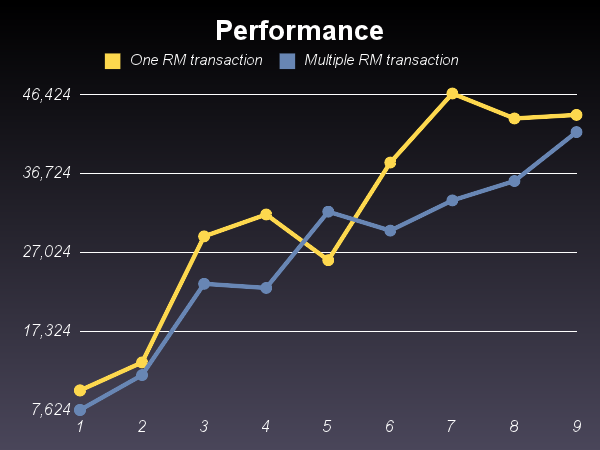
\includegraphics[scale=0.5]{oc_linear.png}
  \caption{Transaction time in microseconds function of the number of clients}
  \label{oneserver}
\end{figure}


\subsection{Distributed servers}

Within a distributed scenario, we try to compare the advantage of having separate RMs running on different server to see the scalability.

\begin{figure}[ht!]
  \centering
	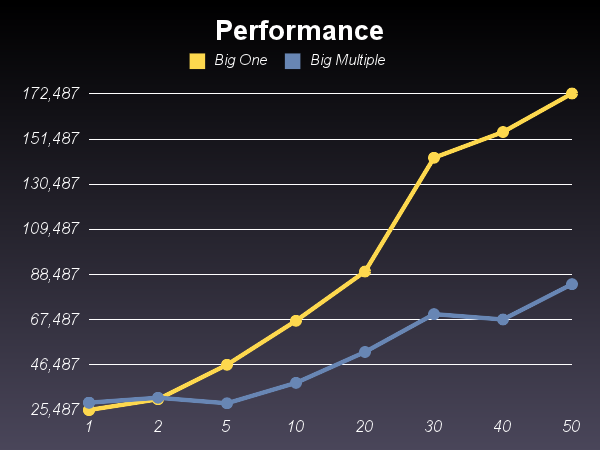
\includegraphics[scale=0.5]{distributed.png}
  \caption{Transaction time in microseconds function of the number of concurrent clients in a distributed environment}
  \label{oneclient}
\end{figure}

In Fig.\ref{oneclient} we see that when we increase the throughput (that is, the number of concurrent clients), a distributed transaction (a transaction involving multiple RMs) has a contained response time even in high throughput ( 26ms when there is two clients, 88ms when there is fifty), but a non distributed transaction response time increases a lot faster. This is due to the fact to the concurrent load is handle by 3 RMs in the distributed case, but only by one in the non distributed case.

An interesting point compared to the non distributed server is that from 1 to 10 concurrent clients, the response time of a distributed transaction is almost constant, contrary to the non distributed server case. This is our \emph{gain} in distributing our system.

However, the difference in performance is not so great, maybe due to the fact that our architecture is not that scalable and independent (the requests \texttt{start}, \texttt{enlist}, \texttt{commit}, \texttt{abort} ..etc.. are executed on each RMs, whatever the transaction is).

\subsection{Replication}

We take advantage of the RMs replication to distribute the \texttt{READ} requests to RMs. Theoretically, it should improve the performance of concurrent READ requests for a resource (car,room or flight), however, it's almost impossible to verify this because we haven't been able to find a test configuration where a RMs read request were the clear bottleneck of the system.


\section{Testing}

The main difficulty of developing a distributed, concurrent system is testing. We choose to make to handle testing manually, with the help of some handwritten scripts to facilitate the deployment of the RMs, Middlewares and Clients.

\begin{itemize}
\item
{\tt launch.sh [tcp/rmi] [car/room/flight/middleware] [port] [.....]}.

It take several arguments to launch each of the service (CarResourceManager,Room,Flight,Middleware or Client), either via TCP or RMI. For each one, it takes a port argument corresponding to the rmiregistry port used for the object binding.
\item
{\tt launch-localhost.sh [tcp/rmi] [portcar] [portroom] [portflight] [portmiddleware]}.

It deploys all the services all at a time on localhost.

\item
{\tt launch-client.sh [tcp/rmi] [host:port]} is used to lunch a client (either RMI or TCP)
allowing fast testing when it's combined with the {\tt input1} file which contains multiple testcases.

\item
{\tt launch-client-automatic.sh}
Launch the automatic (threaded and looped) client. Takes number of concurrent clients , number of loop iteration, expected transaction rate, and transaction type.

\item
{\tt throughput.rb}
Ruby script which use the previous script and execute it for several concurrent clients number. Generate a text file with the average response time of the transactions.

\item
{\tt graph.rb}
Ruby script which takes a specific text file format as input (the same format outputed bu throughput.rb), and generated the appropriate PNG graph.
\end{itemize}

For the replication testing, we also add a \texttt{crash,service,number} command to the client, which randomly crash \texttt{number} instances of the \texttt{service}, thus allowing testing the fault-tolerance of the system.

Unfortunately, manual testing is never sound, and even with scripts, the testing procedure is heavy and error-prone. Thus we can't say that the system is bullet-proof, but it resists to individual RM or Middleware crash ; though in some corner-cases there might be some unwanted write duplications.
\section{Special features}

\begin{itemize}
\item
\emph{Separate RM for each kind of resource.}

In order to allow maximum distribution of the system, we decided early to separate each kind of resource into its own resource manager (the project description and provided codebase were using an unique all-purpose resource manager).
We have factorized the reusable code into an \emph{AbstractResourceManager} class (cf Fig.\ref{uml}).

\item
\emph{Agnostic in term of network protocol (almost)}

Thanks to our \emph{proxy} objects, we have managed to make a code which run either with RMI or TCP has an underlying protocol with almost no modifications.

\item
\emph{Threaded Java Client}

Both RMI and TCP client can launch concurrent requests to the system in addition to simple sequential looped requests.
\end{itemize}
\end{document}
